%!TEX root = ../../main.tex
\usepackage{hyperref}
\chapter{Nutzerzentrierte Umfrage}
\label{chapter:5}

Während dieser Studienarbeit steht die Verbesserung und Restrukturierung der CO2-runter Webseite im Vordergrund.
Dabei soll besonders auf die Nutzergruppe eingegangen werden, um mit dem bereits vorgestellten Prinzip des nutzerzentrierten Designs die Webseite für den Endnutzer ansprechender und interessanter zu gestalten.
Durch dieses Vorgehen soll die Webseite sowohl in den Punkten Design und Nutzerfreundlichkeit, als auch im Allgemeinen verbessert werden.
Das Ziel dahinter ist, dass mehr potenzielle Nutzer gefunden und angesprochen werden, um so zu einem klimabewussteren Denken anzuregen.

Da der Nutzer im Zentrum des Vorgehens steht, werden selbstverständlich Ideen, Kritik und Einflüsse von potenziellen Nutzern der Webseite, aber auch von Menschen im Allgemeinen, über die bisherige Webseite benötigt.
Um diese Kritik und Einflüsse zu sammeln wird im Rahmen dieser Studienarbeit eine nutzerzentrierte Umfrage durchgeführt.
Mithilfe der Umfrage sollen Meinungen, Kritik und Ideen von unparteiischen Personen gesammelt werden, sodass diese im Anschluss ausgewertet werden können und dem Entwicklerteam entscheidende Hinweise darüber bieten, welche Aspekte der aktuellen Webseite größeren Sanierungsbedarf haben bzw.
welche Aspekte bereits ihren Zweck und Wert erfüllen.
In den folgenden Unterkapiteln wird das Vorgehen von der Sammlung der möglichen Fragen der Umfrage, bis hin zur Auswertung der Umfrageergebnisse dokumentiert.

% > Das dann nutzen und eine Umfrage machen wie die Webapp mehr genutzt werden kann und auch verbessert werden kann
% > wie siehts bei mir eigetlich aus aus der User perspektive
% > interaktivere Landing Page für den Nutzer
% > Anregen das er ein Forumlar ausfüllt um zu erfahren wie viel er macht im verlgiech zum avg. User so ?
% > Userzentriertes Vorgehen was ist das
% > Die Ansätze davon erleutern
% > Abwegen was genutzt wird davon
% > Was ist User Zentrietes Vorgehen und was für Verfahren gibt es um die Webseite

\section{Methodik der Umfrage}

%Eine eigene Umfrage zu erstellen und durchzuführen bedeutet viel Aufwand. Besonders die Planung der Umfrage und das Sammeln von Fragen erfordert einen höheren Zeitaufwand als eventuell erwartet.
%In den nächsten beiden Unterkapitel werden die Phasen der Umfrageplanung und -durchführung beschrieben.

Die Methodik der Umfrage bildet das methodische Grundgerüst, das die systematische Erfassung und Analyse von Daten ermöglicht, um präzise Einblicke in die untersuchte Thematik zu gewinnen. In diesem Kapitel werden die spezifischen Vorgehensweisen und Verfahren detailliert erläutert, die im Rahmen der durchgeführten Umfrage angewendet wurden.
Von der Auswahl der Stichprobe über die Gestaltung des Fragebogens bis hin zur Datenerhebung und -auswertung werden die methodischen Schritte transparent dargestellt.

\subsection{Planung der Umfrage}
Zu Beginn jeder Umfrage steht die Planung der Umfrage.
Die Planung ist einer der wichtigsten, wenn nicht sogar der wichtigste, Schritt einer Umfrage, da auf Basis der in der Planung festgelegten Konzepte etc.
die finale Umfrage aufbaut und schlußendlich auch durchgeführt wird.
Dazu wird im Buch \texttt{Umfrage} beschrieben, dass jedes Forschungsprojekt grundsätzlich mit einer Planungsphase beginne.
Darin werden unter anderem die theoretische Fundierung der Forschungsfrage als auch der daraus resultierende Art der Froschung festgelegt.\cite{umfrage:2011}

Die Forschungsfrage wird am Anfang eines Forschungsprojektes bestimmt und steuert das weitere Vorgehen des Projektes. \cite{umfrage:2011}
In unserem Fall bearbeiten wir die Forschungsfragen: "Wie kann man mehr Menschen dazu motivieren, die CO2-runter Webseite zu nutzen?"\ und "Wie kann man klimabewussteres Verhalten im Allgemeinen erzeugen?".

Mit der Forschungsfrage ergibt sich zumeist automatisch auch die Art der Forschung.
Dabei unterscheidet man im Allgemeinen grundsätzlich vier Arten von Untersuchungen:

\begin{itemize}
    \item \textbf{Explorative Untersuchung:} Untersucht man einen Bereich mit seiner Untersuchung bzw. Umfrage, in welchem bisher nur sehr wenige bzw. keine Informationen und Erkenntnisse vorliegen, so handelt es sich um eine explorative Untersuchung. Das Ziel einer explorativen Untersuchung ist es, einen ersten Überblick über den Untersuchungsbereich zu gewinnen und Grundlagenforschung durchzuführen. Häufig wird diese Art der Untersuchung als Umfragenforschungsprojekt als vorbereitende Forschung verwendet. \cite{umfrage:2011}
    \item \textbf{Deskriptive Untersuchung:} Bei einer deskriptiven Untersuchung gibt es bereits ein recht großes Vorwissen. Das primäre Ziel ist hierbei Detailinformationen zu einem Thema zu erlangen. Zusätzlich im Zentrum des Interesses stehen hier Fragen nach der Verteilung bestimmter Merkmale und Merkmalskombinationen,aber auch nach Veränderungen z.B. im Zeitverlauf \cite{umfrage:2011}\ Ergebnisse einer deskriptiven Untersuchung werden höufig in Tabellen präsentiert. Bekannt sind diese aus Printmedien und/oder dem Fernsehen.\cite{umfrage:2011}
    \item \textbf{hypothesentestende bzw. kausalanalytische Forschung:} Sollte man bei einer Untersuchung bereits vor der empirischen Untersuchung Vermutungen über die Ausprägung bestimmter Verteilungen angestellte werden, spricht man von einer hypothesentestenden Untersuchung.\cite{umfrage:2011}
\end{itemize}

Bei unserer Umfrage handelt es sich um eine kausale Untersuchung.
Das liegt daran, dass mit der Umfrage eine Ursache-Wirkung-Beziehung zwischen den Aspekten der Webseite und der Nutzerfreundlichkeit herauszufinden.
Durch die Sammlung der Daten, welche Aspekte der aktuellen Webseite gut oder schlecht bewertet wurden, kann man Hypothesen aufstellen, welche Elemente der Webseite zu einer positiven bzw. negativen Nutzererfahrung führen.\

Bevor die eigentliche Umfrage erstellt wurde, wurden in einem Dokument Fragen gesammelt um einen Fragenkatalog zu erstellen. Der Fragenkatalog dient zur Sammlung möglicher Fragen, damit diese nach der Sammelphase erneut überarbeitet und gewichtet werden können.
Der Fragenkatalog besteht aus insgesamt \textbf{31} Fragen.
Die Fragen wurden in einer Brainstorming-Aktion gesammelt und ohne Ordnung notiert.
Nach der Brainstorming-Aktion wurden die Fragen kategorisiert.
Dabei wurden die folgenden Kategorien erstellt und für die Einordnung der Fragen genutzt:

\begin{itemize}
    \item CO2 Fußabdruck
    \item Motiviation Nutzung
    \item Verbesserung Webseite
    \item aktueller Stand der Webseite
\end{itemize}

Im nächsten Schritt wurden die kategorisierten Fragen bewertet und nach ihrer Wichtigkeit eingeteilt.
Für die Bewertung wurden Ganzzahlen im Interval von 0 (= nicht so wichtig) bis 5 (= muss vorhanden sein) bewertet.
Alle Fragen die mit einer 5 gekennzeichnet wurden, wurden später automatisch mit in die Umfrage aufgenommen.
Von allen 31 Fragen wurden insgesamt 26 mit einer 5 gekennzeichnet und wurden somit 1:1 bzw. in einer ähnlichen Form in die Umfrage aufgenommen.
Selbstverständlich wurden während der Erstellung der Umfrage weitere Fragen hinzugefügt, da der Fragenkatalog lediglich als Orientierung und ersten roten Faden verwendet wurde.\

Nun wurde mit der eigentlichen Erstellung der Umfrage begonnen.
Die Umfrage wurde mithilfe von \href{https://docs.google.com/forms/u/0/}{Google Formulare} erstellt.
Da Google mit Google Formulare eine kostenlose Möglichkeit zum Erstellen von Umfragen mit vielen Features bietet, wurde auf diese Software bei der Erstellung der Umfrage gesetzt.\

Die Umfrage enthält insgesamt 5 Abschnitte.
Die Abschnitte sind hierbei mit Kategorien zu vergleichen, da darauf geachtet wurde, dass ähnliche Fragen innerhalb eines Abschnitts präsentiert werden.
Die Umfrage startet mit einem kleinen Einführungsabschnitt.
Darin werden die Teilnehmenden begrüßt und der Grund der Umfrage wird genauer erläutert.
Es wird ebenfalls darauf hingewiesen, dass es von Vorteil ist, die Originalwebseite aufzurufen.
Dies hat zum einen den Vorteil, dass die Teilnehmer die Webseite live erleben können.
Aber es bietet selbstverständlich auch eine erste Werbung.
Abschließend wird der Teilnehmende in diesem ersten Abschnitt darauf aufmerksam gemacht, dass die Umfrage ungefähr 30min dauern kann und diese anonym durchgeführt wird.
Es wird also weder eine Email, noch andere persönliche Daten für die Teilnahme an der Umfrage benötigt.

Der zweite Abschnitt thematisiert das vorhandene Wissen des Teilnehmers über den CO2-Fußabdruck im Allgemeinen.
Das Ziel dieses Abschnitts ist es, zu erfahren, inwieweit sich der Teilnehmende bereits mit den Themen CO2-Fußabdruck und Klimaschutz beschätigt hat.
Beispielhafte Fragen aus diesem Abschnitt sind zum Beispiel:
\begin{enumerate}
    \item Kennen Sie den Begriff CO2-Fußabdruck?
    \item Haben Sie sich schon einmal Gedanken über ihren CO2-Fußabdruck gemacht?
    \item Wie bewusst sind Sie sich im Allgemeinen über ihren CO2-Fußabdruck?
\end{enumerate}
Im Falle, dass die erste Frage mit \textit{Nein} beantwortet wurde, besteht die Möglichkeit, innerhalb der Umfrage ein zweiminütiges Erklärvideo zum Thema CO2-Fußabdruck anzuschauen.


Abschnitt drei behandelt das Thema \textit{Motivation}.
Innerhalb des Abschnitts steht die Frage im Fokus, wie man Menschen zu klimafreundlicherem Verhalten motivieren und anregen kann.
Zusätzlich soll auch ermittelt werden, was sich Nutzer eines CO2-Rechners von der Webseite erwarten bzw. erhoffen.
In diesem Teil der Umfrage sind zudem häufig Textfelder unter den Antwortmöglichkeiten, damit die Teilnehmer ihre eigenen Anregungen/Ideen/Meinungen zu den Themen kommunizieren können.
Ziel dieses Abschnitts ist es, herauszufinden, was die Nutzer und vor allem (noch) potenzielle Nutzer von der Webseite erwarten und fordern.
Durch das hier erhaltene Feedback kann bei der späteren Implementierung der neuen Features darauf geachtet werden, dem Nutzer gerecht zu werden.
Der Abschnitt beinhaltet zum einen Fragen, die mit \textit{Ja} oder \textit{Nein} beantwortet werden, wie z.B.:
\begin{enumerate}
    \item Sind Sie bereits aktiv dabei, unser Klima zu schützen?
    \item Motiviert es Sie, wenn Sie ihren Fußabdruck mit anderen Nutzern vergleichen können?
    \item Würde ihnen ein Punktesystem helfen, ihren CO2-Fußabdruck häufiger zu berechnen?
\end{enumerate}
Jedoch befinden sich auch Fragen, die mehrere Auswahlmöglichkeiten bieten, um auf die Frage zu antworten.
Beispielhafte Fragen sind hier:
\begin{enumerate}
    \item Welche Anreize könnten Sie dazu motivieren, die Webseite häufiger zu verwenden?
    \item Welche Möglichkeiten müssten eine Webseite ihnen bieten, um unser Klima (noch) aktiver zu schützen?
\end{enumerate}
Dabei stehen sowohl vordefinierte Auswahlmöglichkeiten zur Verfügung, als auch ein Feld, bei welchem die Teilnehmer eigene Antwortmöglichkeiten eingeben können.
Am Ende des Abschnitts besteht für den Teilnehmer die Option, eigene Ideen einzubringen, wie klimafreundlicheres Verhalten erzeugt werden kann.

Innerhalb des nächsten Abschnitts, Abschnitt 4, wird das Thema \textit{Nutzerfreundlichkeit} behandelt.
Hier wird der Teilnehmende bezüglich der Nutzerfreundlichkeit der aktuellen Webseiten befragt.
Zudem soll ermittelt werden, wie die Nutzerfreundlichkeit und das Zurechtfinden auf der Webseite besser gewährleistet werden kann.
Das gewünschte Resultat ist hierbei, dass ein generelles Bild über die Nutzerfreundlichkeit der aktuellen CO2-runter Webseite gewonnen wird.
Zusätzlich sollen durch das Feedback der Teilnehmenden wichtige Punkte gewonnen werden, die im späteren Designprozess der neuen CO2-runter Webseite zum Thema Nutzerfreundlichkeit mit eingearbeitet werden können.
Die Mehrheit der Fragen des Abschnitts sind so gestaltet, dass den Teilnehmern Screenshots aus der aktuellen Webseite präsentiert werden.
Auf dem Screenshot sind die im Fokus stehenden Aspekte der Webseite mit roten Boxen hinterlegt.
Abbildung 5.1 zeigt ein solches Beispiel:
\begin{figure}[h]
    \label{picture-of-screenshot-with-boxes}
    \centering
    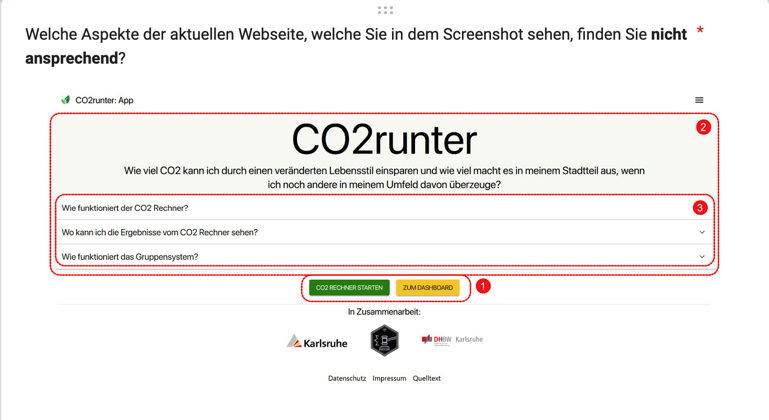
\includegraphics[width=1\textwidth]{images/05/picture_of_screenshot_with_boxes}
    \caption{Frage aus Abschnitt 4, rote Boxen zur Erkennung des Fokus}
\end{figure}

Anschließend werden dem Teilnehmenden Ankreuzmöglichkeiten anhand der Zahlenwerte geboten, um die Frage zu beantworten.
Es gibt auch jedes Mal die Antwortmöglichkeit, die alle Optionen verneint bzw. bejaht.
Sowie die Möglichkeit, eine freie Antwort in Form eines Kurztextes zu verfassen.
Da es innerhalb des CO2-Rechners der Webseite auch die Möglichkeit gibt, bei Fragen eine detaillierte Ansicht zu aktivieren, wird die Notwendigkeit und Meinung nach solch einem Feature abgefragt.
Die detaillierte Ansicht wandelt hierbei eine Frage in mehrere Unterfragen um, bei der detailliertere Fragen zu einem bestimmten Themenbereich gestellt werden.\

Der letzte Abschnitt behandelt das Thema \textit{Design}.
Dabei wird sowohl auf das aktuelle Design der CO2-runter Webseite eingegangen, als auch auf neu erstellte Designprototypen.
Die Teilnehmenden werden aufgefordert, dass alte Design der Webseite zu bewerten.
Im Gegenzug bekommen sie auch Vorschläge zu neuen Designmöglichkeiten, die mit der Software Figma erstellt wurden.
Das Ziel des letzten Abschnitts ist es, herauszufinden, in welchen Teilen der Webseite ein verbessertes Design erwünscht ist.
Dadurch soll gleichzeitig auch die Nutzerfreundlichkeit und die allgemeine Nachfrage nach der CO2-runter Webseite steigen.
Es gibt dabei zwei grundsätzliche Fragetypen innerhalb des Abschnitts: Bewertungsfragen und Ja/Nein/Neutral-Fragen.
Bei den Bewertungsfragen wird dem Teilnehmenden ein Screenshot des relevanten Themas/Bereichs gezeigt.
Anschließend soll der Screenshot bewertet werden.
Ein Beispiel einer solchen Fragen zeigt Abbildung 5.2:
\begin{figure}[h]
    \label{picture-of-evaluation-question}
    \centering
    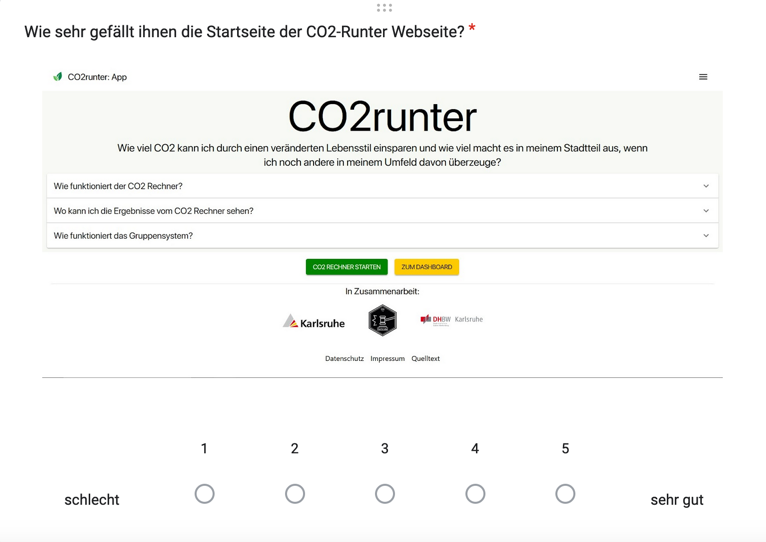
\includegraphics[width=1\textwidth]{images/05/picture_of_evaluation_question}
    \caption{Bewertungsfrage aus Abschnitt 5}
\end{figure}
\subsection{r Fokusdurchführung der Umfrage}

\subsection{Auswahl der Zielgruppe}

\section{Erhebung von Nutzerfeedback}

\subsection{Analyse der Umfrageergebnisse}

\subsection{Identifikation von Herausforderungen und Verbesserungspotenzial}

\section{Userzentrierte Ansätze}

\subsection{Einführung in userzentriertes Vorgehen}

\subsection{Anwendung von Userzentrierten Designverfahren}

\subsection{Evaluierung der effektivsten Ansätze}
